\section{Introduction}
\label{sec:intro}

\paragraph{Motivation and goals}
Distributed robotic applications could transform manufacturing~\cite{pires2000object,gauthier1987interprocess}, transportation~\cite{gerla2014internet,guo2012autonomous}, agriculture~\cite{blender2016managing,r2018research}, delivery~\cite{mosterman2014heterogeneous}, and mapping~\cite{thrun2002robotic}.
Following the trends in cloud, mobile, and machine learning applications, programmability is key in unlocking this potential
as robotics platforms become more open and hardware developers shift to the applications marketplace.
Available domain specific languages (DSL) for robotics are tightly coupled with platforms,
and they combine low-level sensing, communication, and control tasks with the application-level logic
(see~\refsect{related} for more details).
This tight-coupling and the attendant lack of abstraction hinders application development on all fronts---portability, code reuse, and verification and validation (V\&V).

In particular, formal reasoning about a collection of robots communicating, coordinating, and interacting with a physical environment
is complexified by cyber-physical interactions.
Correctness under concurrency and asynchrony are prominent research problems in distributed computing. Correctness under noise, disturbances, and imprecise platform (plant) models is studied intensively by roboticists and control theorists. 
%These areas involve related but entirely different hardware level concepts of control and sensing, and software level concepts of distributed protocols and program interactions. 
The analysis techniques from these communities are based on very different formal models and mathematics, and both would be necessary  to provide satisfactory safety guarantees for  distributed robotic applications.
Our vision is {\em not\/} to combine all of the above in an {\em all encompassing formalism\/}, but to create a language that separates  the concerns to divide and conquer using existing analyses from both communities.

Our goal is to design abstractions and language constructs that separate the \emph{platform-independent} decision and coordination from \emph{platform-dependent} actions.
For example, in an application for distributed package delivery with mobile robots,
the code for waypoint assignment, load-balancing, and handling failures should abstract away implementations of way-point tracking controllers and functions for navigation and communication.
Such application code will be portable, with appropriate platform-specific implementations of these abstractions,
e.g., steering controller for car, thrust controller for a quadcopter, and GPS or indoor localization subroutines.
%
In addition, this separation will enable the joining of analysis techniques.
For example, in this paper we show how symbolic executions for the application program can be combined with model-free and data-driven analysis of the platform-specific controllers.

\paragraph{Approach}
In this paper, we present \lgname: a language and supporting verification and testing tools for programming distributed robotic systems.
\lgname language is designed with following three kinds of users in mind.
\begin{noinditem}
\item \emph{For the application developer}, our \lgname language provides key abstractions (\emph{sensor and actuator ports, distributed shared memory, and synchronous execution})
      to develop robot applications that interact with the the physical environment, and other participating robot programs.
\item \emph{For the V\&V engineer}, the \K-based formal executable semantics we have developed for \lgname and our Z3-based prover,
      can help discharge key invariants of the \lgname applications.
      This verification process also helps identify the \emph{platform-dependent} proof obligations that have to be discharged or validated through simulation and testing.
\item \emph{For the platform engineers} deploying the robot applications, our abstraction makes the \lgname programs portable across platforms. Our high-fidelity \lgname simulator can be used in conjunction with other reachability analysis tools to test and validate the platform-dependent proof obligations.
\end{noinditem}

\begin{figure}[h!]
            \captionsetup{font=scriptsize}

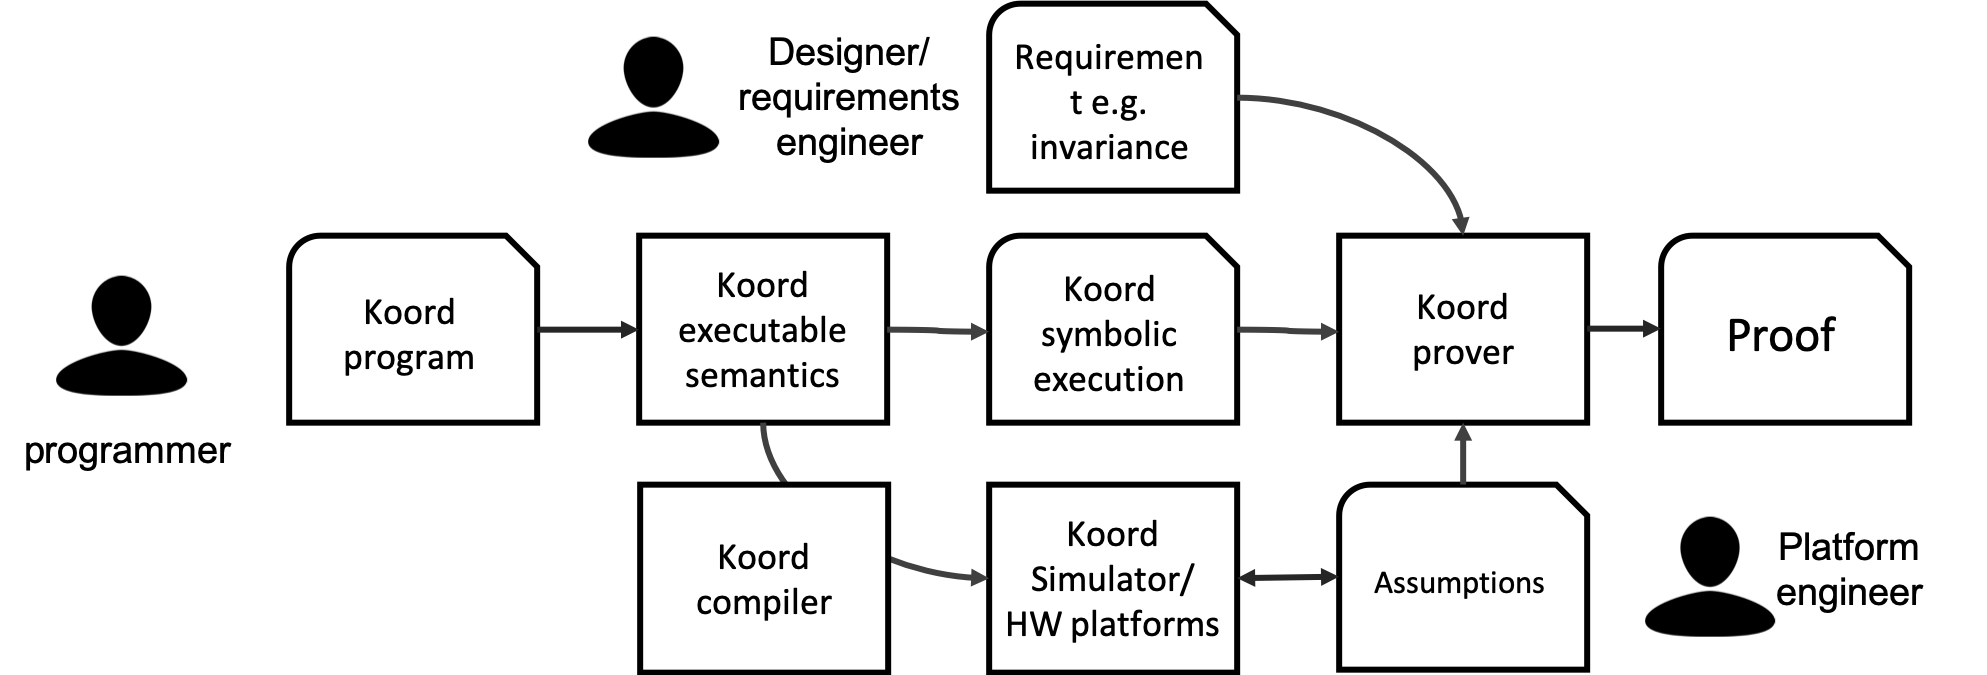
\includegraphics[width=\linewidth]{figs/koorduser.png}
\caption{\lgname language enables programmers to develop distributed robotics applications using a high-level language and prove properties using symbolic executable semantics in \K.
    Platform specific assumptions are abstracted and can be checked using simulations and hardware deployments.}
\label{fig:koorduser}
\end{figure}


\paragraph{Contributions and design decisions}

We have baked-in several abstractions in the design of \lgname to simplify the distributed robotics programming.
Our design of \lgname creates a separation of platform-specific from platform-independent concerns.
The formal semantics of \lgname enables our formal analysis to benefit from this separation of concerns.

\begin{noinditem}
\item We introduce an abstract interface of \emph{sensor} and \emph{actuator ports} through which a \lgname program interacts with its environment.
The program can read from sensor ports to receive updates about its environment;
and it can write to actuator ports to direct the low-level controllers and actuators.
Beyond the names and types of these ports, the abstract interface may specify additional \emph{\portasum{}s} that these ports should satisfy.
Application developers get to use these assumptions to reason about the \lgname application,
while platform engineers ensure that these assumptions are met when implementing the interface for each platform.
These interfaces allow deploying and simulating the same \lgname program on heterogeneous devices without any alteration,
and thus shorten the test-debug-deployment cycle.

\item We provide a \emph{distributed shared memory (DSM)} construct for \lgname applications on different robots to communicate with each other.
This makes \lgname applications very succinct (see examples in \reffig{lineform}),
and raises the level of abstraction for the programmers beyond sockets, message queues, ROS topics~\cite{ros}, etc.
We have developed an implementation of distributed shared memory using UDP messages. %\rg{deployed it across different robotic hardware platforms.}

\item We develop the executable \K semantics~\cite{rosu-serbanuta-2013-k} of \lgname.
To our knowledge this is the first formalization of a programming language for distributed cyber-physical systems which has also been deployed on actual platforms.
Our executable semantics of \lgname in \K, assumes a \emph{synchronous round-by-round computation model for the distributed system}.
Each round lasts for a fixed time period, and all robots synchronize at the beginning of each round.
This synchronous model is a restrictive but standard model for distributed systems~\cite{lynch1996a,attiyawelch}.
While it does not completely eliminate concurrency control, it significantly simplifies programming and verification.
\lgname provides constructs for mutual exclusion as additional mechanisms for concurrency control with shared memory mentioned above.
This model can be implemented under typical synchrony assumptions for multi-robot networks.\footnote{Bounded message delays and clocks with bounded drifts.}

\item We present a \K symbolic execution-based formal verification \sayan{methodology} which does {\em not} require explicit dynamical models of the platform.
In practice, a detailed model of the platform (e.g., dynamic models for cars, wheel friction, engine torque, etc.) may not be available.
The \lgname semantics is \sayan{parameterized} so that any available model or an actual black-box executable for the platform can be plugged in,
and our formal analyses facilitate both inductive invariant checking and state space exploration with black-box dynamics.

\item We identify and separate platform-independent from platform-dependent \emph{proof obligations} derived from our formal analysis of $\lgname$ semantics. We  propose an approach to discharge the former obligations with existing SMT solvers automatically. \rg{On one hand, platform dependent proof obligations can represent the infeasibility of implementing such systems,
when they are difficult to discharge or easily violated in simulation or testing.}
On the other hand, these proof obligations can serve as contracts for sensors, drivers, and operating system modules that are outside the purview  of application developers.
An intended useful outcome of this methodology is a list of formal assumptions for the platform or implementation-specific components such sensors, schedulers, data structures, etc.
\end{noinditem}
%
These choices do leave out issues related to robot failure and dynamic joins and leaves from the current semantics, which could be included in the future.
\rg{However, even without tackling these issues, \lgname tools can handle analysis of behavior and requirements for interesting applications such as distributed formation (a set of robots coordinate to form shapes), task allocation (robots perform a set of tasks in a distributed manner), and mapping (robots collaboratively map obstacles in a given space) as demonstrated in \refsect{verification}.}

%Our semantics facilitates the development of formal analysis tools using techniques such as symbolic post-state computation and bounded-model-checking combined with sensitivity analysis. We present our tools in \refsect{verification}. To our knowledge, this is the only distributed (CPS) system analysis framework with a language semantics component to it, thus reducing the gap between theory and practice.
%Furthermore, as \reffig{krdarch} shows, the components of the $\lgname$ framework interact using interfaces, allowing interchangeability of formal analysis components. For instance Z3 can be replaced by any other SMT solver depending on the user requirements. In fact, by using \K to implement the executable language semantics, we leave room for consistent extensibility of the language to support even more diverse applications.   

%We implemented a suite of benchmarks and used both our formal analysis tools of inductive invariant verification and bounded model checking to verify them or find counter examples. As expected, the state space expands exponentially with the number of agents due to the inherent non-determinism of distributed CPS captured by our system, which is a factor for the running time of both our approaches. However, inductive invariant checking scales much better than explicit state bounded model checking. We also combined the two approaches to analyze and refine a distributed application with a partially known environment model for an automated \emph{traffic} intersection navigation application. Aside from the theoretical and formal analysis, we performed hardware experiments to confirm the assumptions we made while developing the language semantics for $\lgname$. We assume that \begin{inparaenum}\item each participating agent in a system is known \item time taken to execute a computational step can be considered 0 logical time, or negligible compared to $\delta$, \item shared variable updates propagate to all agents immediately \end{inparaenum}. Our hardware experiments support these assumptions. 


%\paragraph{Incomplete model for environment}
%
%
%Allow trade-off between exposing more low level details and simplicity of the language constructs
%


\begin{figure}[h!]
            \captionsetup{font=scriptsize}
\begin{minipage}{0.32\columnwidth}
	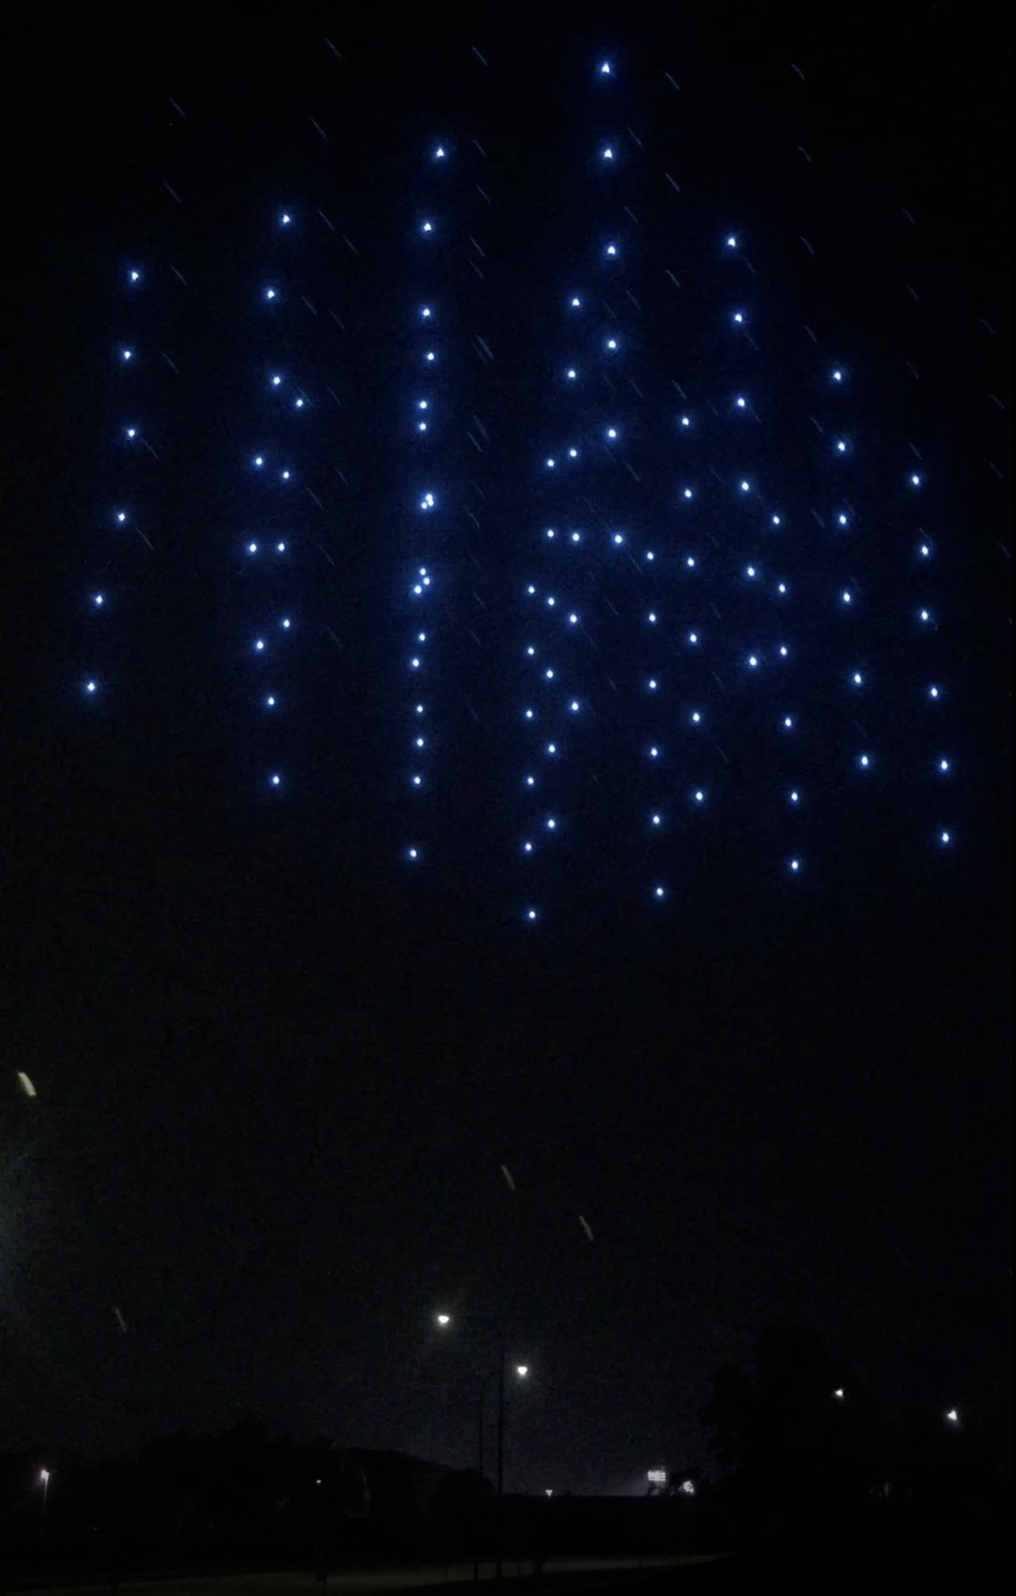
\includegraphics[width=\linewidth]{figs/firefly.png}
\end{minipage}
\begin{minipage}{0.55\columnwidth}
	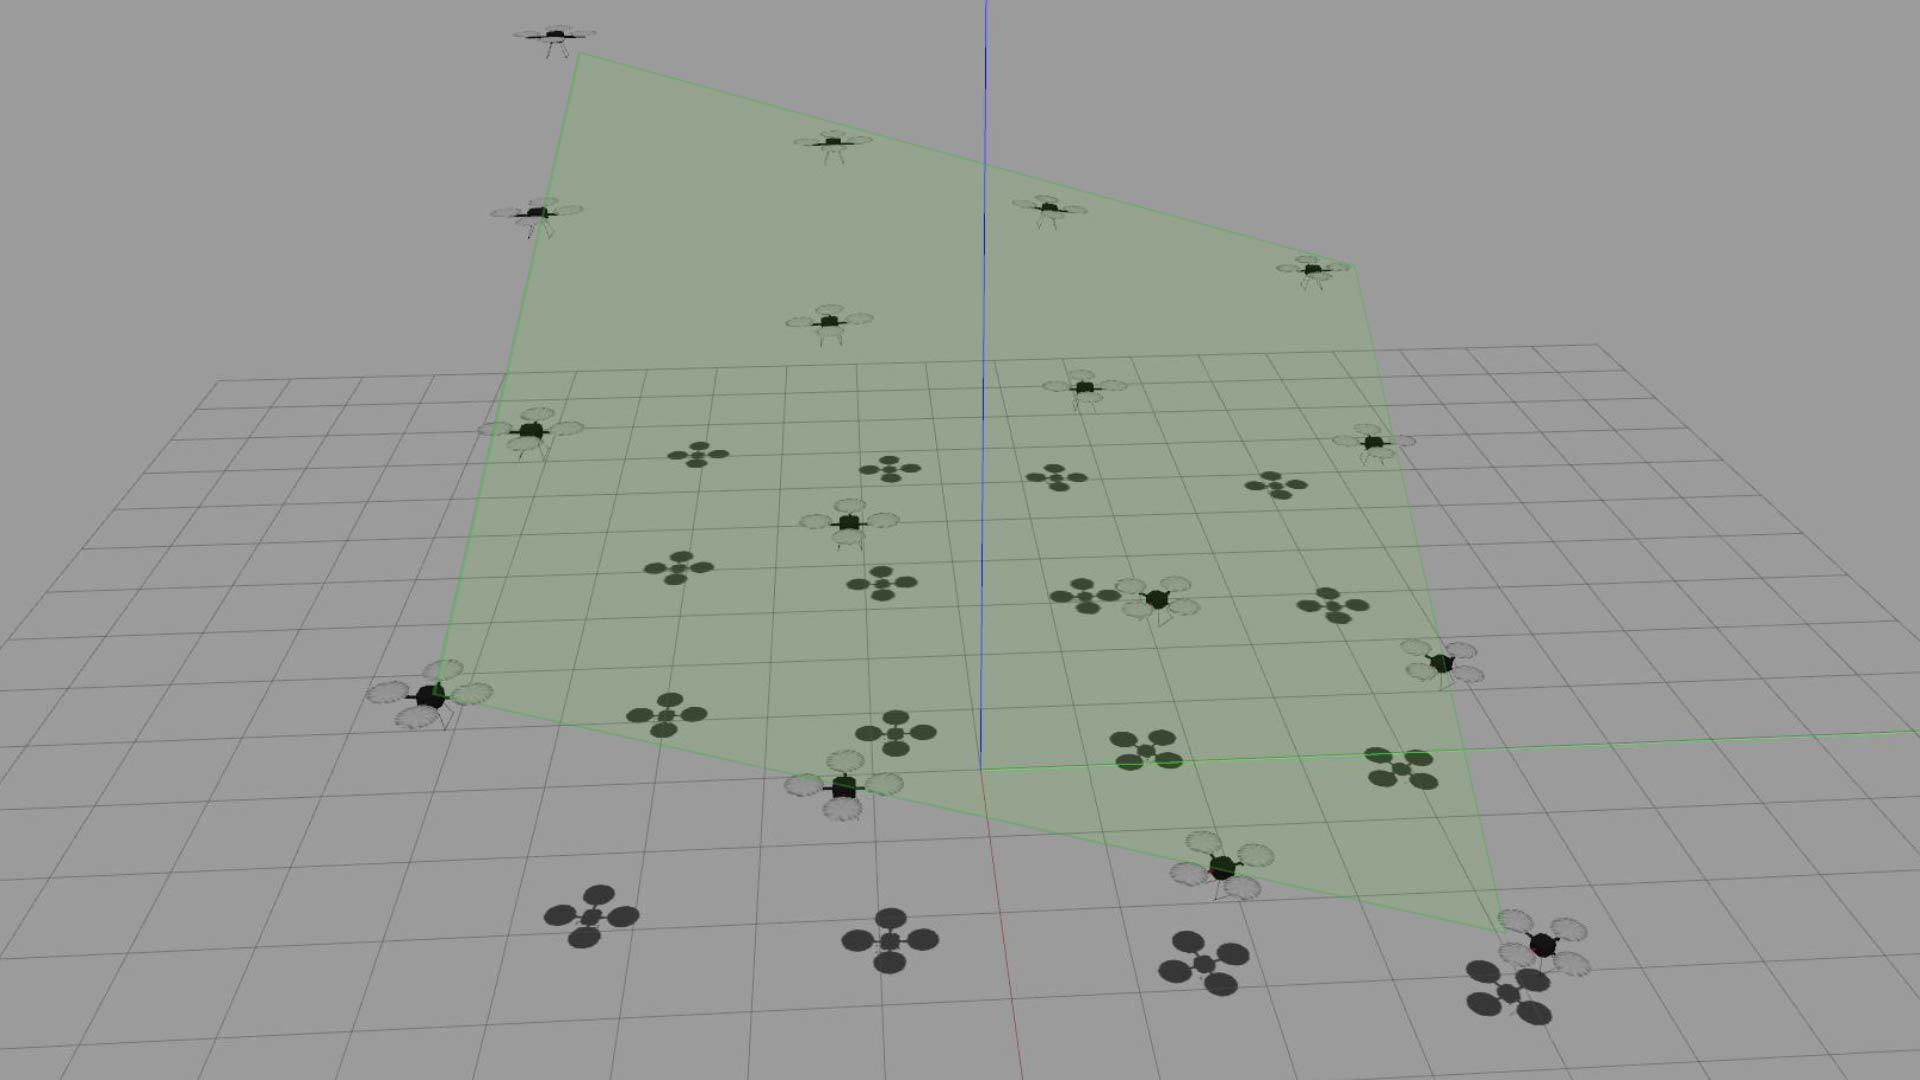
\includegraphics[width=\linewidth]{figs/shapeform_16.jpg}

	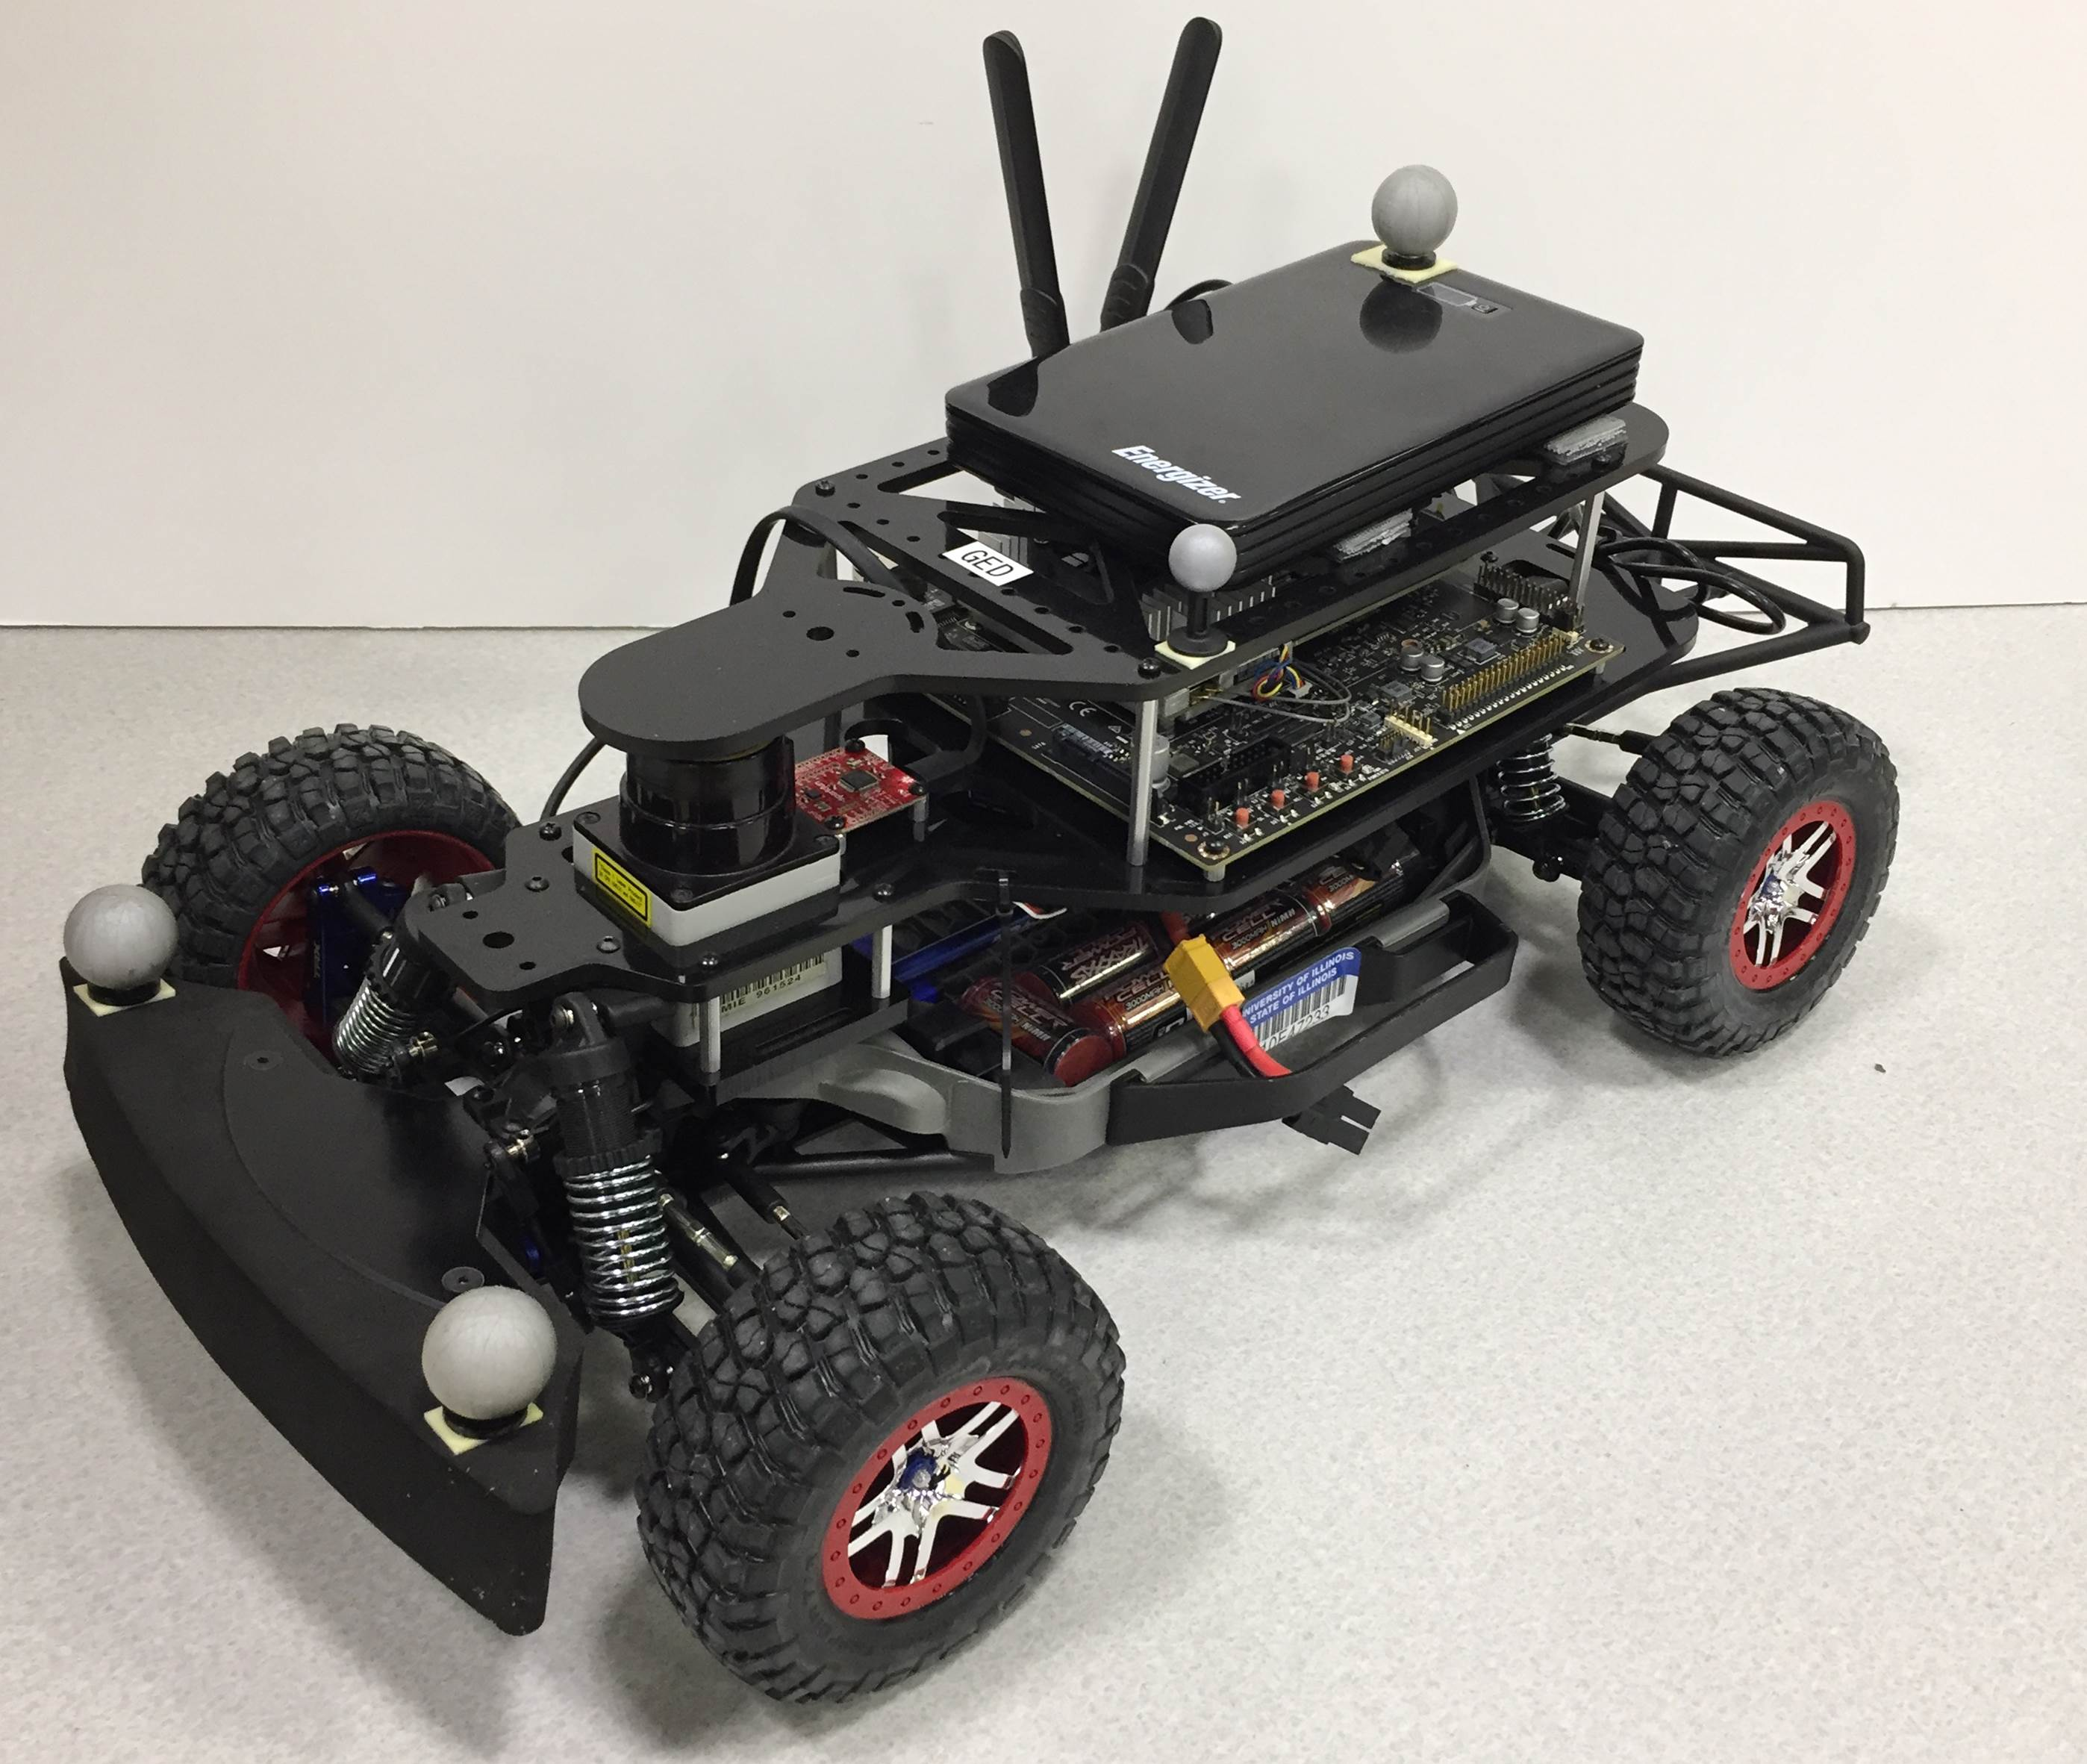
\includegraphics[width=0.42\linewidth]{figs/car.jpg}
	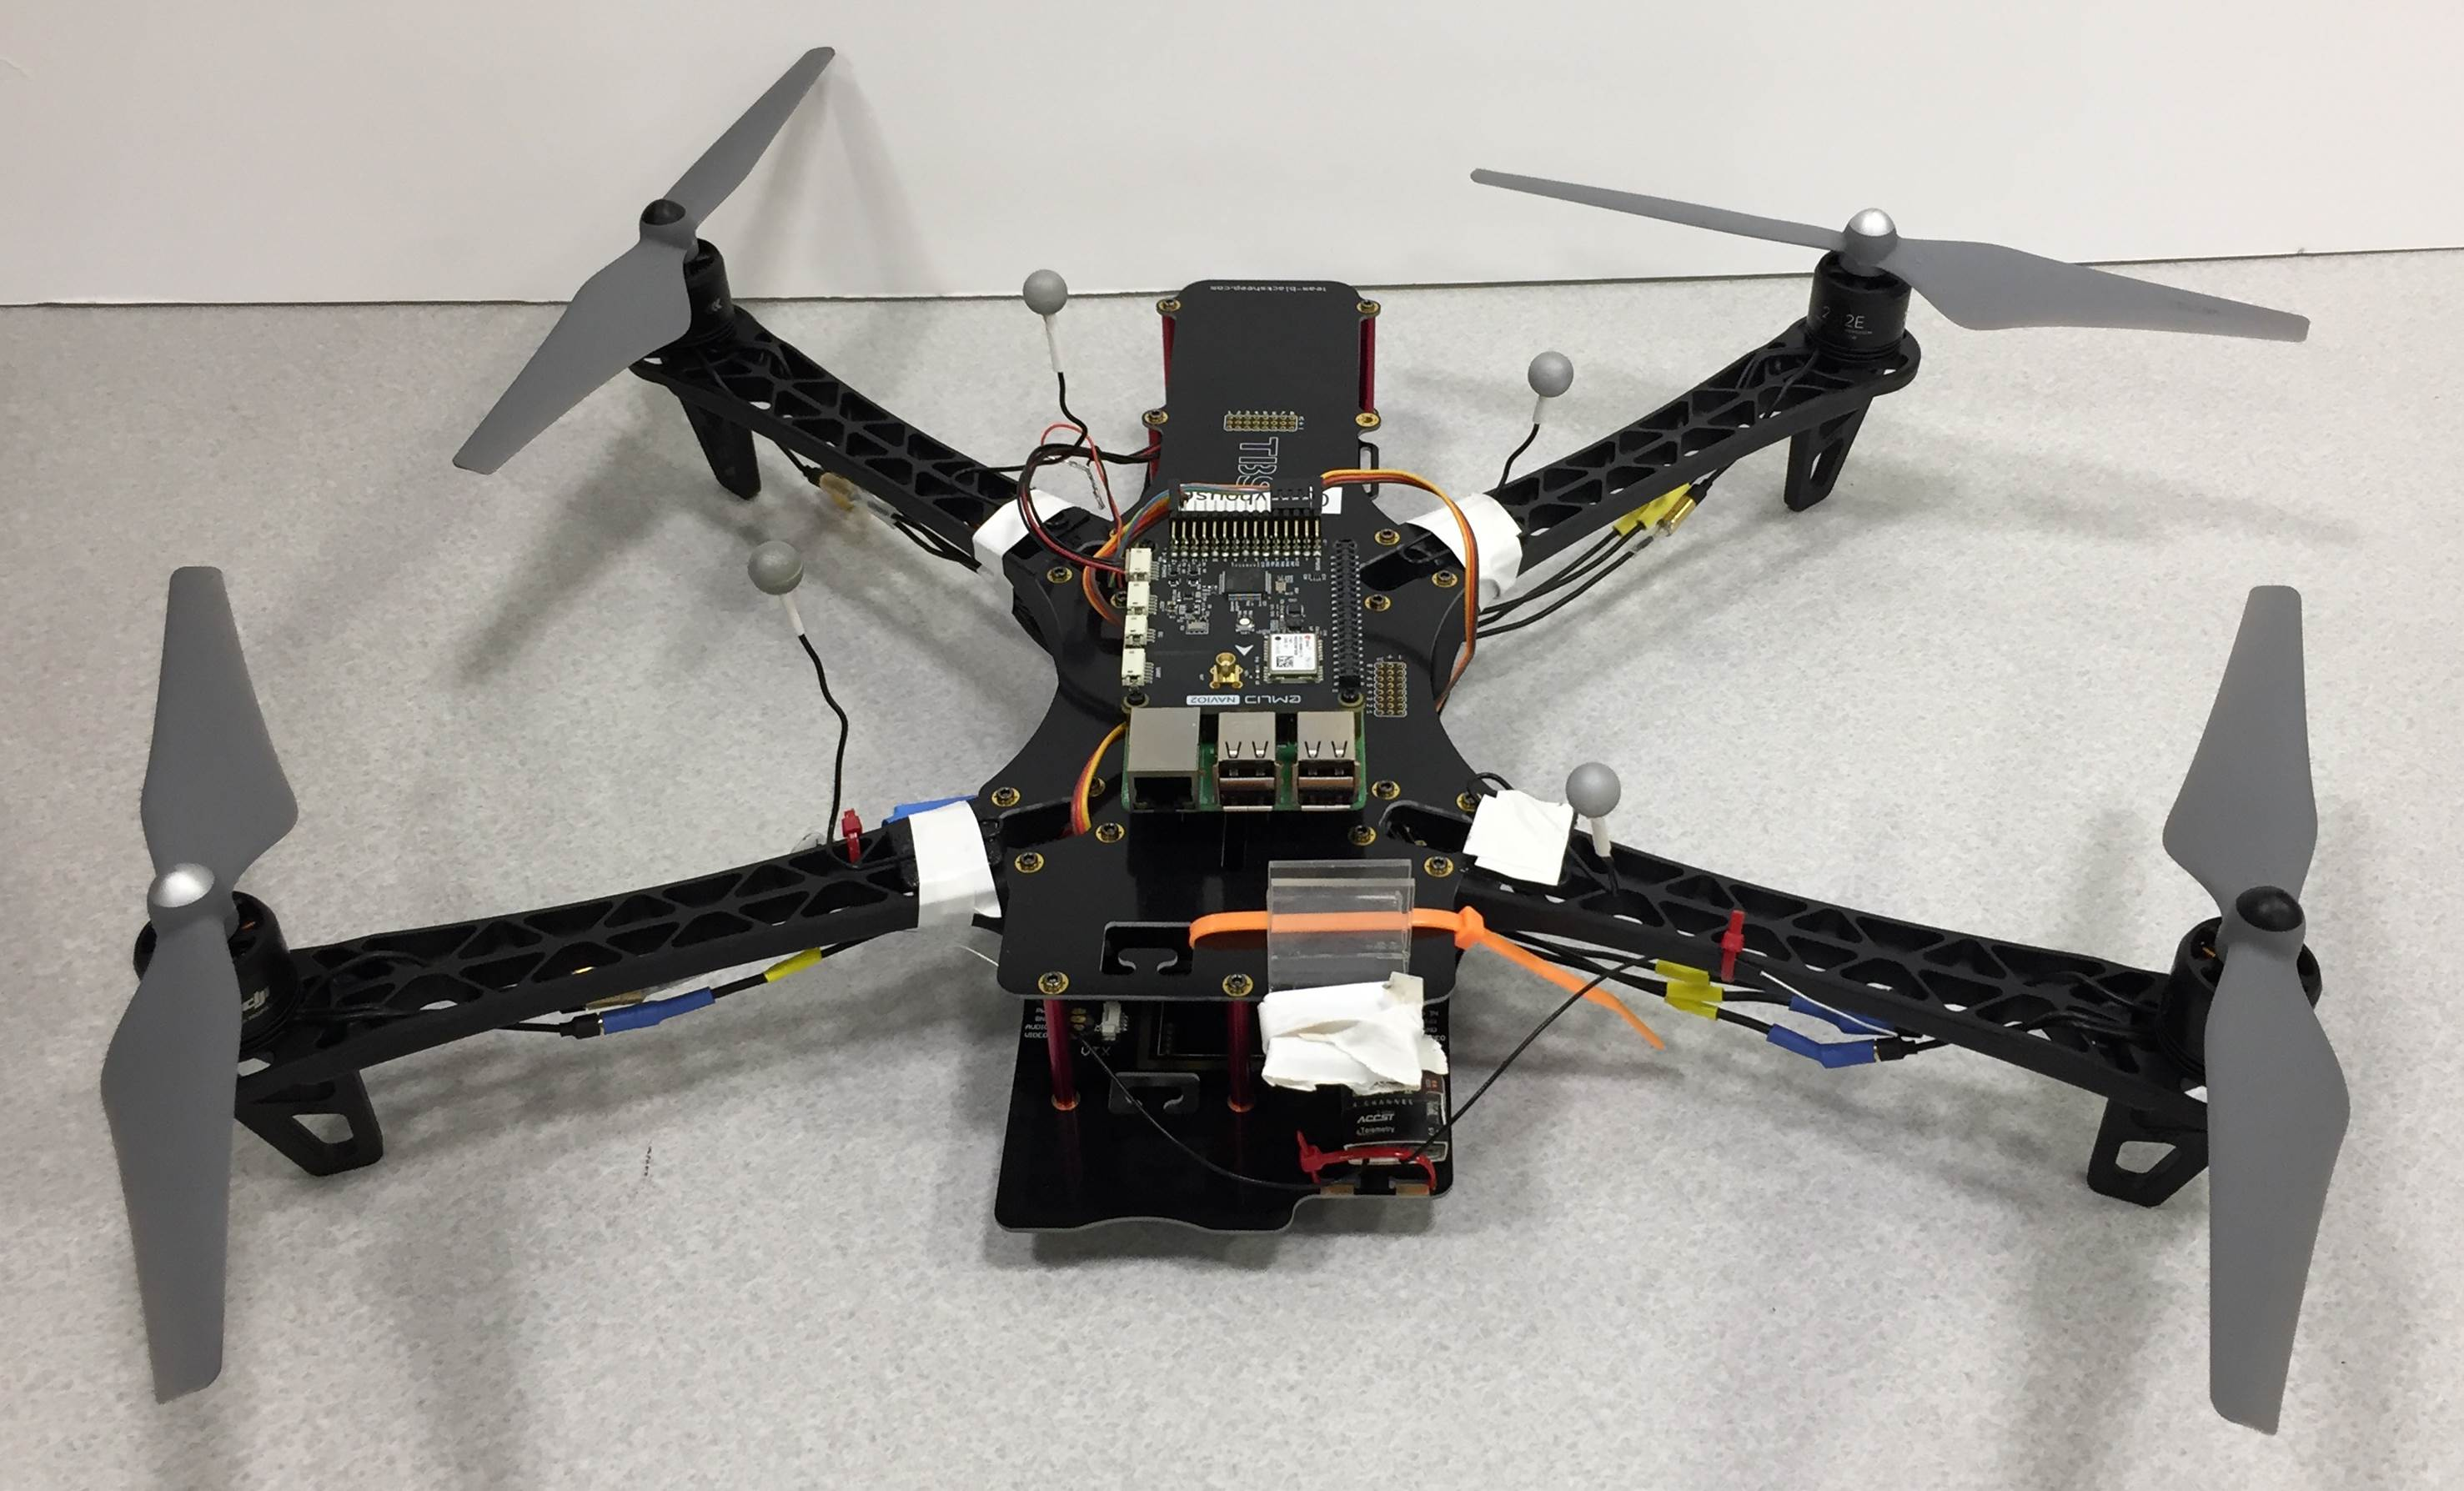
\includegraphics[width=0.56\linewidth]{figs/quad.jpg}
\end{minipage}%
	\caption{
        Swarm formation show by FireFly Inc. (\emph{Left}).
        Simulation of shape formation (\emph{Top Right}).
        Cars and quadcopters we can deploy and test $\lgname$ programs.}
    \label{fig:firefly}
\end{figure}

%\paragraph{Implement trusted run-time environment}

%\marginpar{\scriptsize\sayan{[EuroSys'17] An Empirical Study on the Correctness of Formally Verified Distributed Systems.}}
%\begin{noinditem}
%\item We explored the trade-off between the level of abstraction of the minutiae of multi-robot systems and achieved a simple yet expressive language design enabling a versatile set of multi-robot applications. One of the design choices we made was to abstract away continuous time in language. This required a careful design of the memory model to provide consistency and sychrony guarantees. We achieved distributed shared memory through round-based synchronous message passing. Our compiler translates $\lgname$ programs to Python and a device-independent middle-ware implements the memory model and module interfaces.
%\item We created a simulation environment in Gazebo for testing $\lgname$ applications and validating assumptions, specifically on robot-environment behavior. The simulation environment only differs from a hardware deployment environment in the dynamics models of the physical platforms, but all software components are identical.

%\item Convert pub-sub based message passing to black-box module interface
%\item Wrap around black-box modules (ROS packages) to satisfy assumptions identified in formal analysis : Most technically challenging but difficult to sell
%\item Finally, \sayan{experimental evaluation. What did we learn that can generalize beyond this specific application? How did we extend CyPhyHouse capabilities generally?}
%\end{noinditem}
%\makeatletter
%\let\origsection\section
%\renewcommand\section{\@ifstar{\starsection}{\nostarsection}}
%
%\newcommand\nostarsection[1]
%{\sectionprelude\origsection{#1}\sectionpostlude}
%
%\newcommand\starsection[1]
%{\sectionprelude\origsection*{#1}\sectionpostlude}
%
%\newcommand\sectionprelude{%
%  \vspace{-0.5em}
%}
%
%\newcommand\sectionpostlude{%
%  \vspace{0em}
%}
%\makeatother

%The simulator enables the user to test their discrete event loop with simple motion models to test and debug the application program logic without incurring the cost of hardware deployment in case of buggy programs.
%The simulator also serves as a visualization tool as it can be used to plot the behavior of any program variables, or controller variables. For instance, we implemented a robot \emph{formation} app in $\lgname$, where several robots form a shape in which they are evenly distributed.

%\subsubsection{Other by-products}


%Design and development of the CyPhyHouse open source software system. This includes a discrete event simulator for distributed robotic systems, the application launcher, the run-time logging and monitoring system, and an integrated indoor positioning system. All of these software tools are integrated with our new robot programming language called $\lgname$ and its compiler.


% completely describing the framework.
% the Demonstration of an example application development using CyPhyHouse tools and deployment on a physical system using multiple quadcopters.
%Non-contributions: Spell these out to avoid misdirected criticisms and conflict with overlapping publications.
%\begin{itemize}
%\item Language design
%\item Verification tools.
%\item Low-level controller design for vehicles.
%\end{itemize}

